\documentclass[a4paper, 12pt]{article}

\usepackage{dblfnote}
\usepackage[perpage]{footmisc}
\usepackage{indentfirst}
\usepackage{framed}
\usepackage{tikz}
\usepackage{listings}[language=Python]
\usepackage{float}
\usepackage{subcaption}
\usepackage[square,numbers]{natbib}
%\usepackage{multicol}

\usepackage{setspace}
%\usepackage[skip=2mm, indent=17pt]{parskip}
\onehalfspacing
%\doublespacing


% Custom colors
\usepackage{color}

%\setcounter{secnumdepth}{0}

\usepackage[top=3cm, bottom=3cm, left = 2cm, right = 2cm]{geometry} 
\geometry{a4paper} 
\usepackage{url}
\usepackage{graphicx} 
\usepackage{amsmath,amssymb}  
\usepackage[hidelinks]{hyperref}
\usepackage[labelformat=empty]{caption}
\usepackage{xepersian}
\settextfont{XB Yas}
\usepackage[utf8]{inputenc}

%\usepackage{xepersian}

\DeclareFixedFont{\ttb}{T1}{txtt}{bx}{n}{12} % for bold
\DeclareFixedFont{\ttm}{T1}{txtt}{m}{n}{12}  % for normal

\definecolor{deepblue}{rgb}{0,0,0.5}
\definecolor{deepred}{rgb}{0.6,0,0}
\definecolor{deepgreen}{rgb}{0,0.5,0}

\newcommand\pythonstyle{\lstset{
		language=Python,
		basicstyle=\ttm,
		morekeywords={self},              % Add keywords here
		keywordstyle=\ttb\color{deepblue},
		emph={MyClass,__init__},          % Custom highlighting
		emphstyle=\ttb\color{deepred},    % Custom highlighting style
		stringstyle=\color{deepgreen},
		frame=single,                         % Any extra options here
		showstringspaces=false
}}


% Python environment
\lstnewenvironment{python}[1][]
{
	\pythonstyle
	\lstset{#1}
}
{}

% Python for external files
\newcommand\pythonexternal[2][]{{
		\pythonstyle
		\lstinputlisting[#1]{#2}}}

% Python for inline
\newcommand\pythoninline[1]{{\pythonstyle\lstinline!#1!}}




\begin{document}	
	\noindent
	\begin{minipage}[c]{5cm}
		\baselineskip=.7cm
		\begin{flushright}
			درس : مباحث ویژه در داده‌کاوی
			\\
			دانشجو :
			امیرمحمد خرازی
			\\
			شماره دانشجویی :
			40152521002 
			\\
			استاد درس :  
			\href{mrezghi.ir}{دکتر منصور رزقی آهق}
		\end{flushright}
	\end{minipage}
	\hfill
	\begin{minipage}[c]{3cm}
		\begin{center}
			\href{modares.ac.ir}{
				
\includegraphics[width=2cm]{logo.png}}
		\end{center}	
	\end{minipage}
	\\[1mm]
	\hrule depth .5mm \relax
	\begin{flushright}
		تمرین دوم
		\hfill
		دانشکده علوم ریاضی ، گروه علوم کامپیوتر، گرایش داده‌کاوی
		\\
		\vspace{5mm}
		گیت‌هاب درس (
		\href{https://github.com/A-M-Kharazi/Special-Topics-in-DataMining-TMU.git}{لینک}
		)
		\hfill
		گیت‌هاب این تمرین (
		\href{https://github.com/A-M-Kharazi/Special-Topics-in-DataMining-TMU/tree/main/Homeworks/HW%202}{لینک}
		)
	\end{flushright}
	
	\hrule depth .5mm\relax
	
	%\tableofcontents
	%\newpage
	
	\section*{اطلاعات اضافی}
	برای اطلاعات بیشتر لطفا به گیت‌هاب  مراجعه نمائید:
	
	\begin{center}
		\href{https://github.com/A-M-Kharazi/Special-Topics-in-DataMining-TMU.git}{گیت‌هاب}
	\end{center}

	روش‌ و کد به اندازه توان گزارش نوسی شده است و نتایج هر کدام از الگوریتم ها در آن مشخص است :
	
	
	در مورد الگوریتم
	\lr{Spectral Clustering}
	، این الگوریتم را از پایه (یعنی بدون کمک 
	\lr{sklearn}
	)
	و با توجه به الگوتریم کتاب زکی،در صفحه 459 نوشته ام
	.
	
	گراف مورد نیز به دو روش 
	\lr{RBF}
	و 
	\lr{KNN}
	نیز به صورت دستی و مرحله مرحله حساب شده است. 
	
	تنها بخشی از الگوریتم 
	\lr{Spectral Clustering}
	که از sklearn
	استفاده می‌شود بخش آخر آن برای مشخص کردن خوشه‌های نهایی است. 
	
	در این میان تنها بخشی از سوال تمرین که باقی مانده است، درست کردن ماتریس شباهت با استفاده از 
	\lr{OMP}
	است.
	
	بخش های دیگر آن یعنی بدست آوردن ماتریس لاپلاسین با استفاده از این ماتریس شباهت و ادامه آن تا بدست آوردن نتایج نهایی آورده شده است ولی از آنجایی که ماتریش شباهت بدست آمده، با 
	omp 
	درست نشده است، این بخش از سوال پاسخ داده نشده است. 
	
	می‌توانید برای بررسی بیشتر، گزارش کد را مطالعه فرمائید.
	
	اطلاعات کامل تر شامل نحوه انجام الگوریتم ها و دیگر همه در کد آورده شده است.
	
	نتایج نیز در آنجا قابل مشاهده است.
	
	
	بدلیل حجم زیاد فایل 
	\lr{output}
	های آن حذف شده است تا در گیت‌هاب بهتر قرار بگیرد. 
	
	لطفا در صورت نیاز آن‌ها را اجرا کنید. 
	
	برای هر مدل (
	\lr{kmeans}
	و غیره
	)
	و همچنین در 
	\lr{Spectral Clustering}
	با هر نوع گراف 
	(rbf 
	
	و غیره)
	تصاویری مانند شکل زیر 
	ایجاد میشوند. 	
	
	\begin{center}
		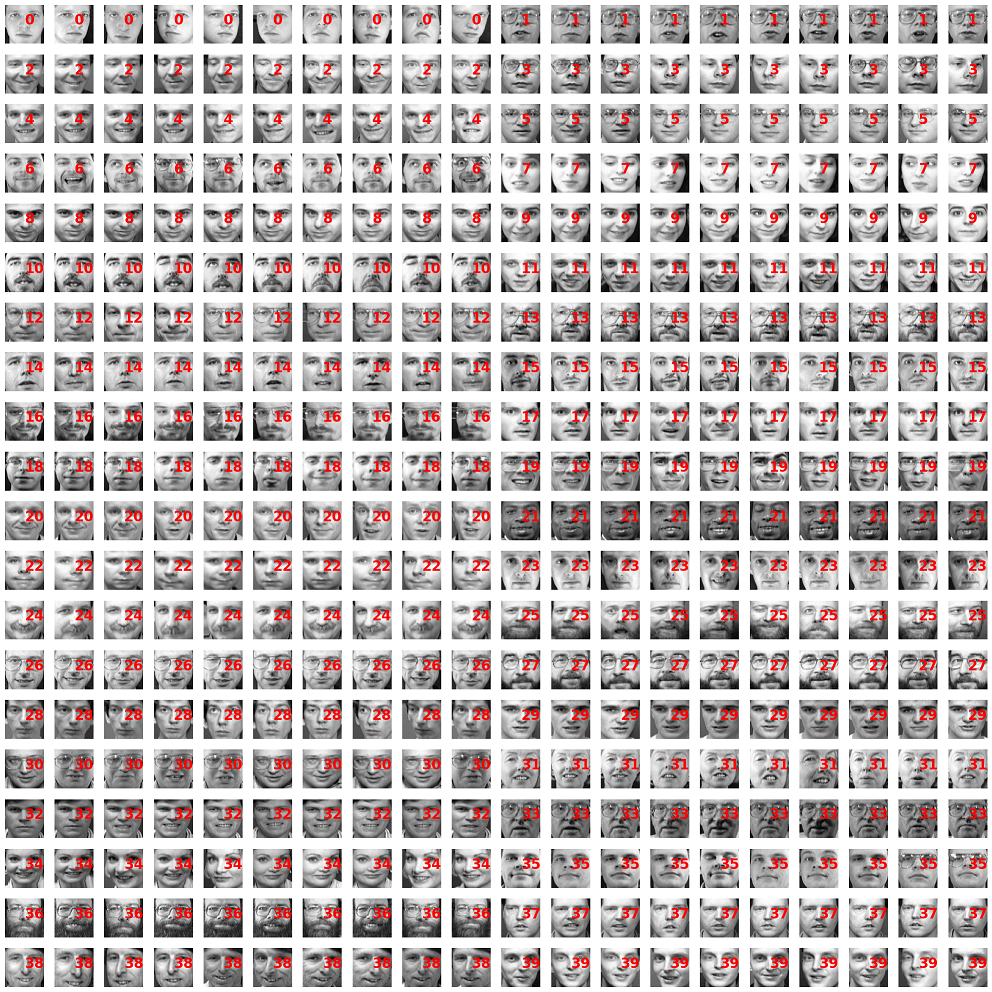
\includegraphics[scale=0.5]{fig1.png}
	\end{center}

\textbf{هر سلول را در کد اصلی اجرا کنید}\\
\textbf{بعضی از خروجی ها برای کمتر کردن حجم فایل پاک شده اند}
\end{document}


